In this chapter we want to give an short overview of current DG methods solving the \MA equation. We focus on two recent methods \cite{BGN+2011, Neilan2014} in particular which later use as our reference DG methods.

\section{State of the Art for Discontinuous Galerkin Methods} % for the \MA equation}

The most natural attempt for a formulation of a DG method solving the \MA equation is to exploit the equations
\begin{align}
	\myIntX {\Omega} {\mydet {D^2 u} v} = \myIntX \Omega {fv} \qquad \text{ for all test functions } v. \label{eq: naiv ansatz}
\end{align}

In 2008 B\"ohmer investigated this approach for $C^1$ elements in \cite{Boehmer2008}. He derives a general $C^1$ method and shows statements on its stability and consistency. 
He reduces The convergence analysis to the linearised case \cite[Section 9]{Boehmer2008}, and thereby discovers and exploits a connection between the weak and strong linearised forms: For $C^1$ elements these operators even coincide meaning the diagram in Figure \ref{fig: fe diagram} commutes.
\begin{figure}[H]
			\begin{center}
		\usetikzlibrary{matrix}

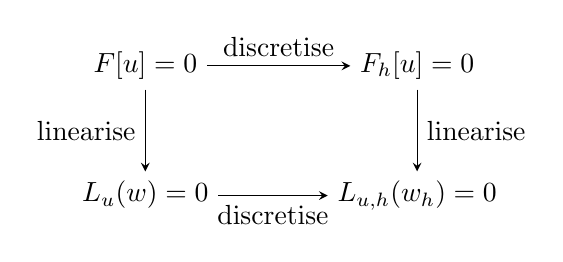
\begin{tikzpicture}[scale =2]
  \matrix (m) [matrix of math nodes,row sep=3em,column sep=4em,minimum width=2em]
  {
     F[u]=0 & F_h[u] =0 \\
     L_u(w) =0 & L_{u,h}(w_h)=0 \\};
  \path[-stealth]
    (m-1-1) edge node [left] {linearise} (m-2-1)
            edge node [above] {discretise} (m-1-2)
    (m-2-1.east|-m-2-2) edge node [below] {discretise} (m-2-2)
    (m-1-2) edge node [right] {linearise} (m-2-2);
\end{tikzpicture}
		\end{center}

	\caption{An abstract commuting diagram about the relation between weak and strong linear operators.\\ The analytical \MA operator is hereby denoted by $F:=\detHess u -f $ and its linearisation $L_u(w) = -\nabla \cdot (\cofHess u \nabla w)$ (cf. Section \ref{sec: linearisation}). $F_h[u]=0$ denotes the discretised formulation, for B\"ohmer's method this is given by \eqref{eq: naiv ansatz}. The diagram is taken from \cite[Fig 2.2]{FGN2013}}
	\label{fig: fe diagram}	
\end{figure}
However, B\"ohmer's ansatz has two major disadvantages. 
First we cannot shift the high derivatives onto the test functions using integration by parts, thus we have to handle the high derivatives. Secondly \eqref{eq: naiv ansatz} seems to work only for elements in $C^1(\Omega)$ which are more complex than the usual $C^0$ elements. B\"ohmer claims that \quoting{We require FEs in $C^1$, since for FEs in $C^0$ we did not see a possibility to handle the interior variational crimes. The standard interplay between the weak and strong form is impossible for fully nonlinear problems and \emph{excludes, e.g. discontinuous Galerkin methods.}}\cite[p. 1214]{Boehmer2008}.

Indeed the diagram in Figure \ref{fig: fe diagram} does not commute for less regular spaces and Brenner et al. make this inconsistency responsible for the failure of $C^0$ methods\cite{BGN+2011}. Their idea is to improve the discretised formulation by adding DG terms to force consistency between the linearisation of the discrete problem and the linearisation of the continuous problem.

\subsection{A $C^0$ Penalty Method }\label{sec: Brenner method}

In this section we present the just mentioned method of Brenner et al. \cite{BGN+2011}. Let $u$ denote the exact solution of the \MA equation. 
At the beginning we take a look at $L_{u,h}(w_h)$ given in Figure \ref{fig: fe diagram}, namely the discretisation of the linearisation of \eqref{eq: naiv ansatz} at the exact solution $u$.

After implying weak boundary conditions the linearisation at $u$ of the left-hand side of \eqref{eq: naiv ansatz} can be derived exactly as in the proof of Theorem \ref{thm: linearisation} leading to a mapping $L_{u,h}$ defined by
\begin{align}
\langle L_{u,h}(w),v\rangle =& -\myIntX {\Omega} {\nabla \cdot \left( \mycof {D^2 u } \nabla w \right) v} 
+ \sigma \sum_{e \in \edgesb} \myIntS {e} {\frac 1 {|e|}{w}{g}}.
%=& \int_{\Omega} \left( \mycof {D^2 u } \nabla w \right) \nabla v. 
\label{eq: linearOperator}
\end{align}

That corresponds to calculating $L_{u,h}$ by first going to the right and then down on the diagram in Figure \ref{fig: fe diagram}. Let us now check what happens if we want to calculate $L_{u,h}$ going first down and then to the right.
We already calculated the linearisation of the \MA equation in Theorem \ref{thm: linearisation} and now have to analyse its variational form. We suppose $w \in H^3(\Omega; \triang) \cap H^1(\Omega)$ and the test functions $v \in H^2(\Omega; \triang) \cap H^1(\Omega)$. Due to integration by parts it holds
\begin{align*}
  -\myIntX  \Omega { \nabla \cdot (\mycof{D^2 u} \nabla w) v}
  	=& \myIntX  \Omega { (\mycof{D^2 u} \nabla w) \cdot \nabla v} \\
  	 &	- \sum_{e \in \edgesb} \myIntS e { \mycof{D^2 u} \nabla w \cdot \mathbf n \; v}.
%  	 + \sigma \sum_{e \in \edgesb} \myIntS {e} {\frac 1 {|e|}{w}{g}}.
\end{align*}
Adding again the weak boundary conditions and an additional term to symmetrise we obtain the variational form of the linearisation
\begin{align}
	\langle L^B_{u}(w),v\rangle 
	    =& \myIntX  \Omega {(\mycof{D^2 u} \nabla w) \cdot \nabla v} \nonumber \\
	    	&- \sum_{e \in \edgesb} \myIntS e { \jump{ \mycof{D^2 u} \nabla w} v} 
	    	- \sum_{e \in \edgesb} \myIntS e { \jump {\mycof{D^2 u} \nabla v} w} \nonumber \\
	    	& + \sigma \sum_{e \in \edgesb} \frac 1 {|e|} \myIntS {e} {{w}{g}}. \label{eq: var of linearisation}
\end{align}
We observe a discrepancy between $L^B_{u}$ and $L_{u,h}$. To overcome this, Brenner et al. rewrite the original nonlinear naive ansatz \eqref{eq: naiv ansatz} to obtain a nonlinear operator $F$ which can be written as the sum of $L^B_{u}$ and a remaining mapping $R$, i.e.
\begin{align}
	\bilin {F (u+w)} v = \bilin {L^B_{u}w} v + \bilin {Rw} v. \label{eq: brenner entwicklung}
\end{align}
Their approach yields the following method: Find $u_h \in V_h$ such that
\begin{align}
\begin{split}
	&\myIntX {\Omega} {\left(f-\mydet {D^2_h u_h}\right) v_h} 
	+ \sum_{e \in \edgesi} \myIntS e { \jump{ \average{\mycof{D^2 u_h} } \nabla u_h } v_h} \\
	&- \sum_{e \in \edgesb} \myIntS e { \jump{ \average{\mycof{D^2 u_h} } \nabla v_h } (u_h -g)} 
	+ \sigma  \sum_{e \in \edgesb} \frac 1 {h_e} \myIntS e { (u_h -g)v_h}  = 0 \; \forall v_h \in V_h. \label{eq: brenner method}
\end{split}
\end{align}
To analyse this method they choose the ansatz and test space $V_h$ to be the space of continuous functions being piecewise polynomials up to degree $k$ for a $k \geq 3$ and assume the \MA problem has strictly convex solution $u\in H^s(\Omega)$ for $s>3$. %Then they are able to derive stability of the linearisation of their operator. 

The key for the convergence proof is a fixed point argument: %They already derived an expansion of the finite element operator in \eqref{eq: brenner entwicklung}. 
%With this at their hand they define a mapping . 
They define a mapping $\mathcal M_h$ such that its fixed point is the solution to their finite element method. 
%The choice of their $\mathcal M$ has two important properties. At first, its fixed point is the solution to their finite element. At second, $\mathcal M$ is chosen in such a way that its contraction property almost follows directly from a contraction property of $R$.
Using the Banach fixed point theorem they can show existence of a fixed point of $\mathcal M$ in $V_h$ and further locate it within an arbitrary small set. This idea is adopted in Section \ref{subsec: comparison brenner}, when we compare this method to a newly derived DG method. Fortunately, their convergence proof also yields an error estimate for their numerical solution:
\begin{theorem}[Error Estimate{\cite[Theorem 3.1 and 3.2]{BGN+2011}}]\label{thm: error estimate brenner}
	There exists an $h_0(\sigma) > 0$ such that for $h \leq h_0(\sigma)$ there exists a solution $u_h$ to the penalty method \eqref{eq: brenner method}. Moreover, if the exact solution $u \in W^{s,\infty}$ with $s>3$ then holds
	\begin{align*}
%		\norm{u-u_h}_{1,h} \lesssim (1+\sigma) h^{l-1} \norm{u}_H
		\norm{u-u_h}_{L^2(\Omega)} \lesssim (1+\sigma)^2 
		                        \left(h^{l} \norm{u}_{H^l(\Omega)} + (1+ | \ln h |^{\frac 1 2 }) h^{2(l-2)} \norm{u}_{H^l(\Omega)} \right)
	\end{align*}
where $l=\min\{k+1,s\}$. 
\end{theorem}
This theorem ensure almost optimal convergence orders provided a smooth solution and the polynomial degree $k\geq 3$. Otherwise the given bound does not converge to zero given $h \rightarrow 0$. However, their numerical results suggest optimal convergence rates for $k=2$.\\
This approach has a drawback. In order to find $u_h$ one has to solve the nonlinear system resulting from \eqref{eq: brenner method}. To present numerical results Brenner et al. make use of Newton's method to solve their example problems. 
To obtain a good initial guess they use a rather complex procedure: They inquire a vanishing moments method which internally again solves a nonlinear systems based on Newton's method. The starting point required by this internal Newton solver is calculated using a nested iteration.

In \cite{Neilan2014} Neilan introduces another DG method. During the presentation of his numerical results Neilan claims that the $C^0$ penalty method fails to converge for the test case $u = -\sqrt{2 - x_1^2 - x_2^2 }$ and $f = \frac 2 {{2 - x_1^2 - x_2^2}^2}$ which lacks $H^2$ regularity. 
In chapter \ref{ch:NumericalResults} we provide some numerical experiments for a nested iteration variant of this method and our computations confirm Neilan's claim, see also Test \ref{test sqrt}. In general we shall see, the presented method is more appropriate for classical solutions, Brenner et al. say they plan to address less regular solution in future work. 


\subsection{A Finite Element Method based on a Discrete Hessian} \label{subsec: disrete Hessian} \label{sec: FEM discrete Hessian}

In \cite{Neilan2014} Neilan generalises a finite element method that Lakkis and Pryer presented in \cite{LP2011}.
The crux of this idea is the notion of a \emph{discrete Hessian}. 
While the Hessian of the exact solution fulfils as we have seen in Lemma \ref{la: integration by parts Frobenius}
	\begin{align}
		\myIntX  \Omega { (D^2 u : B)} = 
			- \myIntX  \Omega { \left(\nabla \cdot B\right) \cdot \nabla u} 
			+ \myIntS {\partial \Omega}  {B \nabla u \; \mathbf {n}} \qquad \forall B \in [H^1(\Omega)]^{d \times d}, \label{eq: part int hessian}
	\end{align}
the piecewise derived Hessian $D_h^2 v$ of $ v \in V_h$ for not so regular ansatz spaces $V_h$ does not inherit this property. Considering that most weak formulations are based on an integration by parts approach, it stands to reason that a discretisation of the Hessian should also have this property. To create such a discretisation Neilan integrates \eqref{eq: part int hessian} piecewise on every triangle and rewrites the edge terms by a combination of jump and averages leading to
	\begin{align}
		\myIntX  \Omega { (D^2 u : B)}
		=& - \myIntX  \Omega { \left(\nabla \cdot B\right) \cdot \nabla u} \nonumber \\
			&+ \sum_{ e \in \edgesi} \myIntS e { \jump {\average B \nabla u }}
			+ \sum_{ e \in \edges} \myIntS e {  \jump{B \average {\nabla u} }}  \qquad \forall B \in \Sigma_h. \label{eq: part int hessian omega}
	\end{align}
Observing that the last step admits test functions $B$ being only piecewise smooth, Neilan suggests the ansatz space $V_h = \mathcal{P}_h^k \cap H^1(\Omega)$ and the test space $\Sigma_h = [\mathcal{P}_h^k]^{d \times d}$.

Substituting in \eqref{eq: part int hessian omega} $\nabla u$ across the edges with its numerical counterpart, namely the numerical trace chosen as $\laverage \nabla u \raverage$ one has
	\begin{align}
		\myIntX  \Omega { (D_{DH}^2 u : B) }
%		&= - \myIntX  \Omega { \left(\nabla \cdot B\right) \cdot \nabla u}
%		+ \sum_{ e \in \edgesi} \myIntS e {  \jump {\average B \nabla u } }
%				+ \sum_{ e \in \edges} \myIntS e { \jump {B \average {\nabla u} }}  \nonumber \\
		&= - \myIntX  \Omega { \left(\nabla \cdot B\right) \cdot \nabla u}
				+ \sum_{ e \in \edges} \myIntS e {  \jump{B \average {\nabla u} }}.	
	\end{align}
Applying once more integration by parts for a Frobenius product on every triangle in the right-hand side integral results in
	\begin{align}
		\myIntX  \Omega { (D_{DH}^2 u : B) }
		=& \myIntX  \Omega { D^2_h u: B }
			-\sum_{ e \in \edgesi} \myIntS e {  \jump {\average B  \nabla u }}
			- \sum_{ e \in \edges} \myIntS e { \jump {B \average {\nabla u} }}\nonumber \\		
			&+ \sum_{ e \in \edges} \myIntS e {  \jump {B \average {\nabla u} }}		\nonumber \\
		=& \myIntX  \Omega { D_h u: B}
			 -\sum_{ e \in \edgesi} \myIntS e {  \jump {\average B  \nabla u }	}.
	\end{align}

Hence, we are able to define the discrete Hessian.
\begin{definition}[Discrete Hessian] \label{def: discrete Hessian}
	The discrete Hessian $D_{DH}^2 u$ of a function $u$ is the unique function satisfying
	\begin{align}
		\myIntX  \Omega { (D_{DH}^2 u : B_h) }
		= \myIntX  \Omega { D^2_h u: B_h}
			 -\sum_{ e \in \edgesi} \myIntS e {  \jump {\average {B_h} \nabla u }}\qquad \forall B_h \in \Sigma_h. \label{eq: discrete hessian}
	\end{align}
\end{definition}

Even though the Hessian is symmetric, in general the discrete Hessian is owing to the face terms not necessarily symmetric. Neilan suggests to replace the ansatz space $\Sigma_h$ by a space of symmetric matrices. Without having this explicitly verified he assumes the analysis given in \cite{Neilan2014} would carry through.\\
Note that for a discontinuous $\Sigma_h$ the computations for $D_{DH}^2 u$ reduce to purely local efforts. For piecewise constant space $\Sigma_h$ the discrete Hessian $D_{DH}^2 u$ can even be computed explicitly.

The next natural step is to plug the newly deduced Hessian into the original \MA PDE resulting in the method: Find $u_h \in V_h$ such that

\begin{align}
		\myIntX  \Omega { \left(\mydet{D_{DH}^2 u_h} - f \right) v_h} = 0 \qquad \forall v_h \in V_h, \label{eq: neilan eq1}
\end{align}
where as in \eqref{eq: discrete hessian}
	\begin{align*}
		\myIntX  \Omega { (D_{DH}^2 u_h : B_h) }
		= \myIntX  \Omega { D^2_h u_h: B_h}
			 -\sum_{ e \in \edgesi} \myIntS e {  \jump {\average {B_h} \nabla u_h }}\qquad \forall B_h \in \Sigma_h.
	\end{align*}

Neilan proceeds analogously to the proof of the well-posedness of the method mentioned in the previous Section \ref{sec: Brenner method}. At the beginning he expands the nonlinear mapping at the exact solution $u$ and then uses an analogous mapping $\mathcal M$ to obtain convergence with the Banach fixed point theorem. Note that the new notion of a discrete Hessian makes the estimates of this unconventional linearisation hard to handle. The linearisation used in the other $C^0$ penalty method is more common and hence the arguments for deriving estimates for the linear part were already well known.
He ends up with the following error estimation:
\begin{theorem}[Error Estimate {,\cite[Theorem 4.2.]{Neilan2014}}] \label{thm: error estimate Neilan}
	Let $u$ be the convex solution to the \MA equation and suppose $u$ to be in the Hölder space $C^{k+3,\alpha}$ for $\alpha \in (0,1)$. Further let $\partial \Omega \in C^\infty$ and $V_h = \mathcal P^k_h \cap H^1(\Omega)$ with $k\geq3$. Then there exists a $h_0$ such that for all $h > h_0$ there exists a solution $u_h \in V_h$ to \eqref{eq: neilan eq1} with
	\[
		\norm{u-u_h}_{1,h} \leq C h^k, 
	\]
	where $C$ is a constant independent of $h$ and $\norm{\cdot }_{1,h}$ is the mesh-dependent discrete semi-norm 
	\[
		\norm{v}_{1,h}^2 = \norm {\nabla v }^2_{L^2(\Omega)} + \sum_{e \in \edges} |e| \norm {\average {\nabla v}}^2_{L^2(e)}.
	\]
\end{theorem}
The norm $\norm {\cdot}_{1,h}$ is equivalent to the norm $\eNorm{\cdot}$ on $V_h$ due the fact that $V_h$ only contains continuous functions.

Albeit Neilan cannot prove any further relaxations, his numerical experiments suggest that his method even works for smaller polynomial degrees and problems whose solution lacks $H^2$ regularity. 
\\However, for $k=1$ he has to add an additional penalty term to obtain convergence. Thus, for piecewise affine functions $u_h \in V_h :=\mathcal P_h^1(\Omega) \cap W^{1,\infty}(\Omega)$ he instead solves:
\begin{align}
		\myIntX  \Omega { \left(\mydet{D_{DH}^2 u_h} - f \right) v_h} 
			+ \eta \sum_{e \in \edgesi} |e| \myIntS e { \jump{ \nabla u_h} \jump{\nabla v_h}}
		= 0 \qquad \forall v_h \in V_h, \label{eq: neilan eq1 + jump}
\end{align}
where
	\begin{align*}
		\myIntX  \Omega { (D_{DH}^2 u_h : B_h) }
		= \myIntX  \Omega { D_h u_h: B_h}
			 -\sum_{ e \in \edgesi} \myIntS e {  \jump {\average {B_h} \nabla u_h }}\qquad \forall B_h \in \Sigma_h \tag{\ref{eq: discrete hessian}}.
	\end{align*}
for $\Sigma_h = \mathcal P^0_k(\Omega)$ and $\eta$ is an additional penalty parameter which Neilan chooses to be 50 in his numerical tests.

We check the performance of this algorithms later in chapter \ref{ch:NumericalResults}.
